\documentclass[border=4pt]{standalone}
\usepackage{tikz}
\usetikzlibrary{arrows.meta, calc}
\usepackage{amsmath, amssymb}

% ── Palette ──────────────────────────────────────────────────────────────────
\definecolor{gnnblue}{RGB}{70,130,190}
\definecolor{gnnfill}{RGB}{210,228,248}
\definecolor{bpgreen}{RGB}{60,155,90}
\definecolor{bpfill}{RGB}{210,240,215}
\definecolor{filmorange}{RGB}{210,120,40}
\definecolor{fillfill}{RGB}{252,235,205}
\definecolor{iogray}{RGB}{100,100,100}
\definecolor{iofill}{RGB}{235,235,235}

%
%  LAYER MAP  (all y values in TikZ units = cm)
%  ───────────────────────────────────────────────────────────────────────────
%  y = 6.0   FiLM Generator box
%  y = 4.6   FiLM horizontal branch routing  ← γ,β labels go here
%  y = 3.0   Main pipeline  (all blocks & arrows)
%  y = 1.6   Formula annotation strip        ← Λ'=…  Λ''=… labels go here
%  y = 0.4   Passthrough routing             ← Λ / Λmid bypass lines
%  y = -0.9  Legend
%
%  x positions:
%   syn/llr: -4.2   gnn1: 0.0   add1: 3.0
%   bp1: 6.2        gnn2: 9.8   add2: 13.0
%   bp2: 16.2       hard: 19.0  out: 20.7
%   film: 4.9       pest: 0.5
% ───────────────────────────────────────────────────────────────────────────

\begin{document}
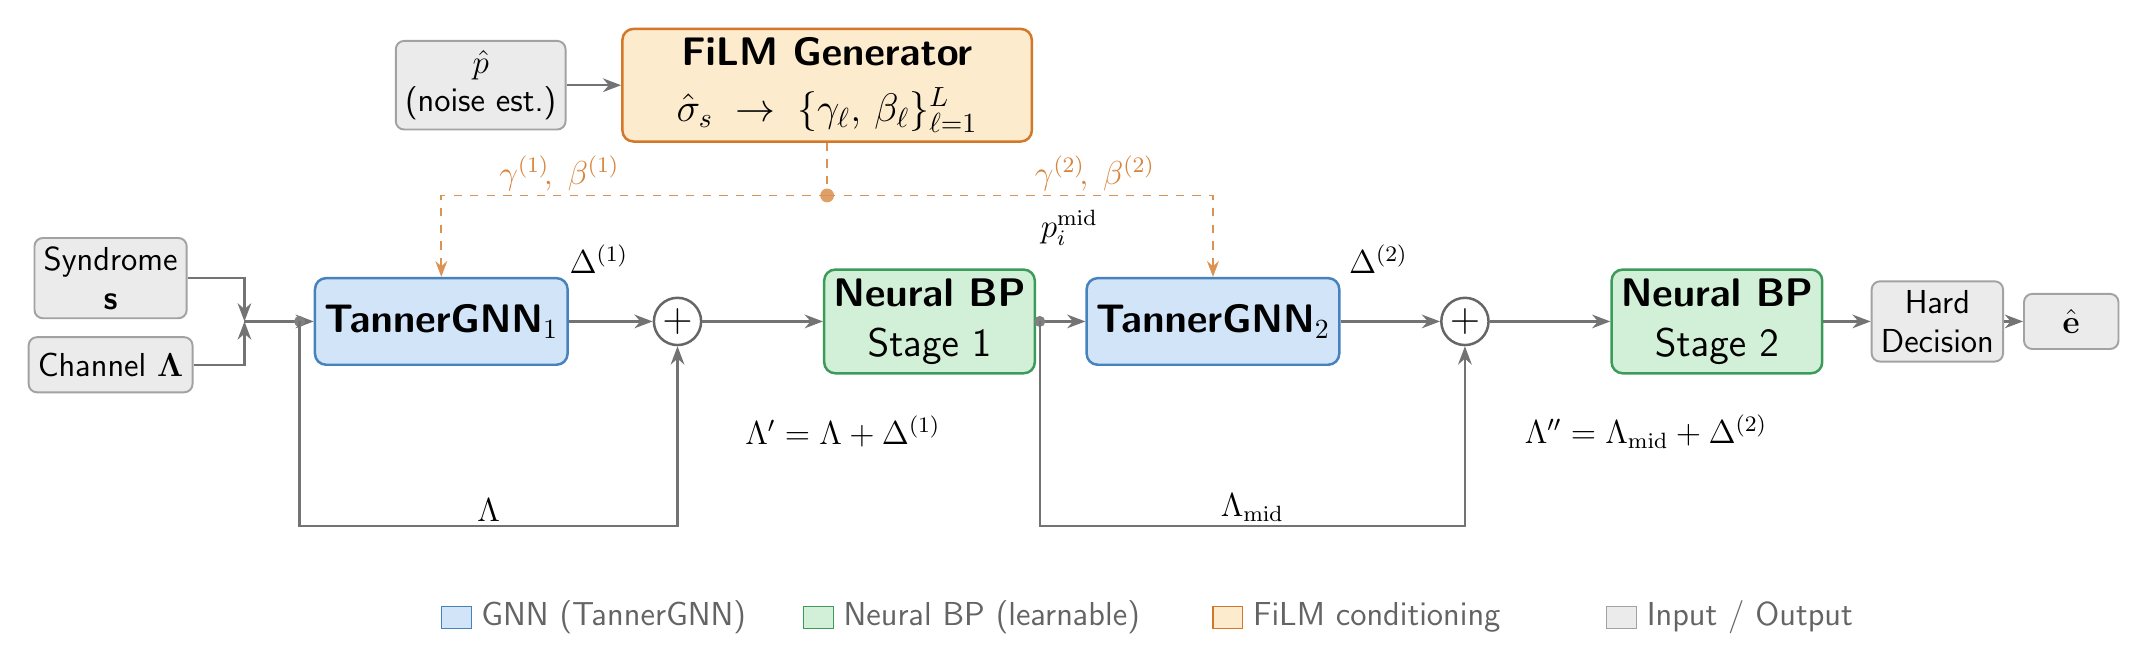
\begin{tikzpicture}[
    >=Stealth,
    font=\sffamily\Large,
    gnn/.style  = {rectangle, draw=gnnblue, fill=gnnfill, line width=0.9pt,
                   rounded corners=4pt,
                   minimum width=2.6cm, minimum height=1.1cm, align=center},
    bp/.style   = {rectangle, draw=bpgreen, fill=bpfill, line width=0.9pt,
                   rounded corners=4pt,
                   minimum width=2.5cm, minimum height=1.1cm, align=center},
    film/.style = {rectangle, draw=filmorange, fill=fillfill, line width=0.9pt,
                   rounded corners=4pt,
                   minimum width=5.2cm, minimum height=1.1cm, align=center},
    io/.style   = {rectangle, draw=iogray!60, fill=iofill, line width=0.7pt,
                   rounded corners=3pt, minimum width=1.2cm, minimum height=0.7cm,
                   align=center, font=\sffamily\large},
    hd/.style   = {rectangle, draw=iogray!60, fill=iofill, line width=0.7pt,
                   rounded corners=3pt, minimum width=1.6cm, minimum height=0.7cm,
                   align=center, font=\sffamily\large},
    plus/.style = {circle, draw=black!60, fill=white, line width=0.9pt,
                   minimum size=0.6cm, inner sep=0pt},
    arr/.style  = {->, thick, black!55},
    farr/.style = {filmorange!80, dashed, semithick},
    lbl/.style  = {font=\sffamily\large, inner sep=1.5pt}
]

% ════════════════════════════════════════════════════════════════════════════
%  PIPELINE NODES  (y = 3.0)
% ════════════════════════════════════════════════════════════════════════════

\node[io]   (syn)  at (-4.2, 3.55) {Syndrome\\\textbf{s}};
\node[io]   (llr)  at (-4.2, 2.45) {Channel $\boldsymbol{\Lambda}$};
\coordinate (join) at (-2.5, 3.00);   % merge point for syn+llr

\node[gnn]  (gnn1) at ( 0.0, 3.0) {\textbf{TannerGNN}$_1$};
\node[plus] (add1) at ( 3.0, 3.0) {$+$};
\node[bp]   (bp1)  at ( 6.2, 3.0) {\textbf{Neural BP}\\Stage 1};
\node[gnn]  (gnn2) at ( 9.8, 3.0) {\textbf{TannerGNN}$_2$};
\node[plus] (add2) at (13.0, 3.0) {$+$};
\node[bp]   (bp2)  at (16.2, 3.0) {\textbf{Neural BP}\\Stage 2};
\node[hd]   (hard) at (19.0, 3.0) {Hard\\Decision};
\node[io]   (out)  at (20.7, 3.0) {$\hat{\mathbf{e}}$};

% ════════════════════════════════════════════════════════════════════════════
%  FiLM GENERATOR  (y = 6.0)
% ════════════════════════════════════════════════════════════════════════════

\node[io]   (pest) at (0.5, 6.0) {$\hat{p}$\\(noise est.)};
\node[film] (film) at (4.9, 6.0)
    {\textbf{FiLM Generator}\\[2pt]
     $\hat{\sigma}_s \;\to\; \{\gamma_\ell,\,\beta_\ell\}_{\ell=1}^{L}$};

% ════════════════════════════════════════════════════════════════════════════
%  MAIN PIPELINE ARROWS
%  – Δ labels: standalone nodes placed ABOVE arrows, yshift large enough to
%    clear box edges; never on-arrow text that can brush a node corner
%  – p_i^mid: standalone node floated high above the bp1→gnn2 gap
% ════════════════════════════════════════════════════════════════════════════

\draw[arr] (syn.east) -| (join);
\draw[arr] (llr.east) -| (join);
\draw[arr] (join)     -- (gnn1.west);
\draw[arr] (gnn1.east)-- (add1.west);   % Δ(1) label below ↓
\draw[arr] (add1.east)-- (bp1.west);
\draw[arr] (bp1.east) -- (gnn2.west);   % p_i^mid label below ↓
\draw[arr] (gnn2.east)-- (add2.west);   % Δ(2) label below ↓
\draw[arr] (add2.east)-- (bp2.west);
\draw[arr] (bp2.east) -- (hard.west);
\draw[arr] (hard.east)-- (out.west);

% Δ(1): above the gnn1→add1 gap, offset high enough to miss both box corners
% gnn1.east=(1.3,3), add1.west=(2.725,3)  → midpoint x=2.0125
\node[lbl, above] at (2.0, 3.55) {$\Delta^{(1)}$};

% Δ(2): above the gnn2→add2 gap
% gnn2.east=(11.1,3), add2.west=(12.725,3) → midpoint x=11.9
\node[lbl, above] at (11.9, 3.55) {$\Delta^{(2)}$};

% p_i^mid: floated clearly above the bp1→gnn2 gap, below FiLM branch level
% bp1.east=(7.45,3), gnn2.west=(8.5,3)  → midpoint x=7.975
% y=3.9 clears all node tops (y=3.55) and stays below FiLM branch (y=4.6)
\node[lbl, above] at (7.975, 3.9) {$p_i^{\mathrm{mid}}$};

% ════════════════════════════════════════════════════════════════════════════
%  FiLM BRANCHES  (y = 4.6 horizontal routing layer)
%
%  Routing: film.south → stem → junction → LEFT horizontal → gnn1.north
%                                        → RIGHT horizontal → gnn2.north
%  No diagonals.  γ,β labels sit ABOVE their horizontal segments, with
%  >1 unit clearance from the vertical descent into each GNN.
% ════════════════════════════════════════════════════════════════════════════

% film.south ≈ (4.9, 5.45).   Branch horizontal y = 4.6.
\coordinate (fjunc) at (4.9, 4.6);

% Stem – no arrowhead
\draw[farr] (film.south) -- (fjunc);
\fill[filmorange!70] (fjunc) circle (2.5pt);   % branch-point dot

% Left branch: horizontal to x=0 then straight down to gnn1.north (0, 3.55)
\draw[->, farr] (fjunc) -- (0.0, 4.6) -- (gnn1.north);

% γ(1),β(1): above the horizontal segment, near its midpoint
% segment runs x=0 → x=4.9; midpoint ≈ x=2.3
% anchor is south so the text sits clearly above the wire
\node[lbl, filmorange!90, above] at (1.5, 4.6)
    {$\gamma^{(1)}\!,\;\beta^{(1)}$};

% Right branch: horizontal to x=9.8 then straight down to gnn2.north (9.8, 3.55)
\draw[->, farr] (fjunc) -- (9.8, 4.6) -- (gnn2.north);

% γ(2),β(2): above its horizontal segment midpoint ≈ x=7.35
\node[lbl, filmorange!90, above] at (8.3, 4.6)
    {$\gamma^{(2)}\!,\;\beta^{(2)}$};

% ════════════════════════════════════════════════════════════════════════════
%  PASSTHROUGH LINES  (y = 0.4 routing layer)
%
%  All routing runs BELOW the main pipeline.  Each line:
%    junction on pipeline → vertical drop to y=0.4
%    → horizontal run → vertical rise into (+).south
%
%  No label is placed on any vertical segment, only on horizontal segments,
%  and only where there is no other horizontal line (different x ranges).
%
%  Λ   bypass: x range [−1.8, 3.0]  at y=0.4
%  Λmid bypass: x range [7.6, 13.0] at y=0.4   (no overlap)
% ════════════════════════════════════════════════════════════════════════════

% ── Λ passthrough ───────────────────────────────────────────────────────────
% Junction on join→gnn1 arrow.
%   join=(-2.5,3), gnn1.west=(-1.3,3)  → pick x=−1.8 (between them)
\coordinate (ljunc) at (-1.8, 3.0);
\fill[black!50] (ljunc) circle (2pt);
% Route: drop → horizontal (x: −1.8→3.0) → rise into add1.south
\draw[arr]
    (ljunc) -- (-1.8, 0.4)            % vertical drop
             -- ( 3.0, 0.4)            % horizontal
             -- (add1.south);          % vertical rise
% "Λ" label above the horizontal segment, away from vertical ends
% midpoint of [−1.8, 3.0] = 0.6
\node[lbl, above] at (0.6, 0.4) {$\Lambda$};

% ── Λmid passthrough ─────────────────────────────────────────────────────────
% Junction just right of bp1.east (7.45,3); pick x=7.6
\coordinate (mjunc) at (7.6, 3.0);
\fill[black!50] (mjunc) circle (2pt);
% Route: drop → horizontal (x: 7.6→13.0) → rise into add2.south
\draw[arr]
    (mjunc) -- ( 7.6, 0.4)             % vertical drop
             -- (13.0, 0.4)             % horizontal
             -- (add2.south);           % vertical rise
% "Λmid" label above the horizontal segment
% midpoint of [7.6, 13.0] = 10.3
\node[lbl, above] at (10.3, 0.4) {$\Lambda_{\mathrm{mid}}$};

% ════════════════════════════════════════════════════════════════════════════
%  FORMULA ANNOTATIONS  (y = 1.6 strip)
%
%  Strictly between the passthrough layer (y=0.4) and the pipeline (y=3.0).
%  Horizontally placed in the GAPS between nodes, offset from ALL vertical
%  lines (passthrough drops/rises and node sides).
%
%  Vertical lines at x = −1.8 (Λ drop), 3.0 (Λ rise), 7.6 (Λmid drop), 13.0 (Λmid rise)
%
%  Formula Λ':  centred at x=5.1  (between Λ-rise at 3.0 and Λmid-drop at 7.6)
%  Formula Λ'': centred at x=15.3 (right of Λmid-rise at 13.0, clear of bp2)
% ════════════════════════════════════════════════════════════════════════════

\node[lbl, align=center] at (5.1, 1.6)
    {$\Lambda' = \Lambda + \Delta^{(1)}$};

\node[lbl, align=center] at (15.3, 1.6)
    {$\Lambda'' = \Lambda_{\mathrm{mid}} + \Delta^{(2)}$};

% ════════════════════════════════════════════════════════════════════════════
%  NOISE ESTIMATOR → FiLM
% ════════════════════════════════════════════════════════════════════════════

\draw[arr] (pest.east) -- (film.west);

% ════════════════════════════════════════════════════════════════════════════
%  LEGEND  (y ≈ −0.9)
% ════════════════════════════════════════════════════════════════════════════

\begin{scope}[shift={(0.0, -0.9)}]
  \fill[gnnfill]   (0.0,0) rectangle (0.38,0.28); \draw[gnnblue]   (0.0,0) rectangle (0.38,0.28);
  \node[lbl, iogray, anchor=west] at (0.45, 0.14) {GNN (TannerGNN)};
  \fill[bpfill]    (4.6,0) rectangle (4.98,0.28); \draw[bpgreen]   (4.6,0) rectangle (4.98,0.28);
  \node[lbl, iogray, anchor=west] at (5.05, 0.14) {Neural BP (learnable)};
  \fill[fillfill]  (9.8,0) rectangle (10.18,0.28);\draw[filmorange](9.8,0) rectangle (10.18,0.28);
  \node[lbl, iogray, anchor=west] at (10.25,0.14) {FiLM conditioning};
  \fill[iofill]   (14.8,0) rectangle (15.18,0.28);\draw[iogray!60](14.8,0) rectangle (15.18,0.28);
  \node[lbl, iogray, anchor=west] at (15.25,0.14) {Input / Output};
\end{scope}

\end{tikzpicture}
\end{document}
